
%----------------------------------------------------------------------------------------
%	PACKAGES AND OTHER DOCUMENT CONFIGURATIONS
%----------------------------------------------------------------------------------------



%% immagini
%\begin{figure}[h]
% \centering
% \includegraphics[width=\columnwidth]{diagrammiClassi/gerarchiaPersone}
% \caption{Diagramma delle classi - Gerarchia utenti.}
%\end{figure}

%----------------------------------------------------------------------------------------
%	ASSIGNMENT INFORMATION
%----------------------------------------------------------------------------------------
%% APPUNTI
% È
% \begin{figure}[h]
% \centering
% \includegraphics[width=16cm]{immagini/img1}
% \caption{Descr ~\cite{rif1}.}
%  \end{figure}


\documentclass{report}

\usepackage[utf8]{inputenc}
\usepackage[italian]{babel}
\usepackage{import}
\usepackage{todonotes}
\usepackage{color}
\usepackage{rotating}
\usepackage[hidelinks]{hyperref}
\usepackage{url}
\usepackage{pdfpages}
\usepackage{siunitx}
\usepackage{pdflscape}
\usepackage{subfig}
\usepackage[euler]{textgreek}

\usepackage{enumerate} % Custom item numbers for enumerations
\usepackage{amsmath}
\usepackage{amsfonts}

\usepackage[signatures,swapnames,sans]{frontespizio}

\usepackage{geometry}
\geometry{portrait, margin=3cm}
\usepackage{siunitx}
\usepackage{booktabs}

\renewcommand*\figurename{Figura}

\newcommand{\sub}[1]{\textsubscript{#1}}
\newcommand{\super}[1]{\textsuperscript{#1}}

\newcommand{\Fig}[0]{Fig.}

\usepackage{titlesec}

\titleformat{\chapter}{\normalfont\huge}{}{20pt}{\huge\bfseries}

\linespread{1.1}

\begin{document}
\addtocounter{chapter}{-1}
	\begin{frontespizio}
		\Margini{3cm}{3cm}{3cm}{3cm}
		\Universita{Bergamo}
		\Logo[43.332mm]{unibg-mark}
		\Divisione{Scuola di Ingegneria}
		\Corso[Laurea Magistrale]{Ingegneria Informatica}
		\Titolo{Elettronica e Misure Industriali}
		\Sottotitolo{Relazione esperienze di laboratorio}
		\Punteggiatura{}
		\NRelatore{Prof.}{Prof.}
		\Relatore{Valerio Re}
		\NCorrelatore{Prof.}{Prof.}
		\Correlatore{Massimo Manghisoni}
		\Candidato[1058231]{Giulia Allievi}
		\Annoaccademico{2021--2022}
		\begin{Preambolo*}
			\usepackage[italian]{babel}
			\usepackage[T1]{fontenc}
			\usepackage[utf8]{inputenc}
			\usepackage{microtype}
			\usepackage{lmodern}
			\graphicspath{{img/}}
			
			\renewcommand{\frontinstitutionfont}{\fontsize{14}{17}\bfseries\scshape}
			\renewcommand{\fronttitlefont}{\fontsize{17}{21}\bfseries\scshape}
			\renewcommand{\frontfootfont}{\fontsize{12}{14}\bfseries\scshape}
		\end{Preambolo*}
	\end{frontespizio}



%----------------------------------------------------------------------------------------
%	PAGINA BIANCA
%----------------------------------------------------------------------------------------
\newpage
\null
\thispagestyle{empty}
\newpage

%----------------------------------------------------------------------------------------
%	INDICE
%----------------------------------------------------------------------------------------
\tableofcontents

%----------------------------------------------------------------------------------------
%	PAGINA BIANCA
%----------------------------------------------------------------------------------------
\newpage
\null
\newpage

%----------------------------------------------------------------------------------------
%	INTRO
%----------------------------------------------------------------------------------------
\chapter{Introduzione}
Nelle esperienze di laboratorio si sono realizzati ed analizzati i seguenti circuiti:
\begin{itemize}
\item Esperienza 1: Emitter follower con alimentazione duale; 
\item Esperienza 2: Emitter follower con alimentazione singola; 
\item Esperienza 3: Common emitter amplifier con alimentazione duale e singola; 
\item Esperienza 4: Amplificatore invertente ed integratore con 	\textmu A741.
\end{itemize}
La relazione è suddivisa per tipologia di circuito.
%----------------------------------------------------------------------------------------
%	CIRCUITO 1: EMITTER FOLLOWER	
%----------------------------------------------------------------------------------------
\chapter{Circuito 1: Emitter Follower}
\section{Introduzione} 
Il primo circuito realizzato è l'\textit{Emitter follower}, detto anche \textit{Common collector}. Questo circuito ha un guadagno unitario, infatti la tensione misurata in uscita è uguale alla tensione applicata in ingresso, perciò si comporta come un buffer. Ne abbiamo realizzate due diverse versioni, una con alimentazione duale e una con alimentazione singola. 
\section{Prima versione} % alimentazione duale
La prima versione di \textit{Emitter follower} analizzata è quella ad alimentazione duale. Di seguito si riportano lo schema, l'analisi del punto di lavoro e di piccolo segnale, e le misure effettuate su questo circuito. 
\begin{figure}[h]
\centering
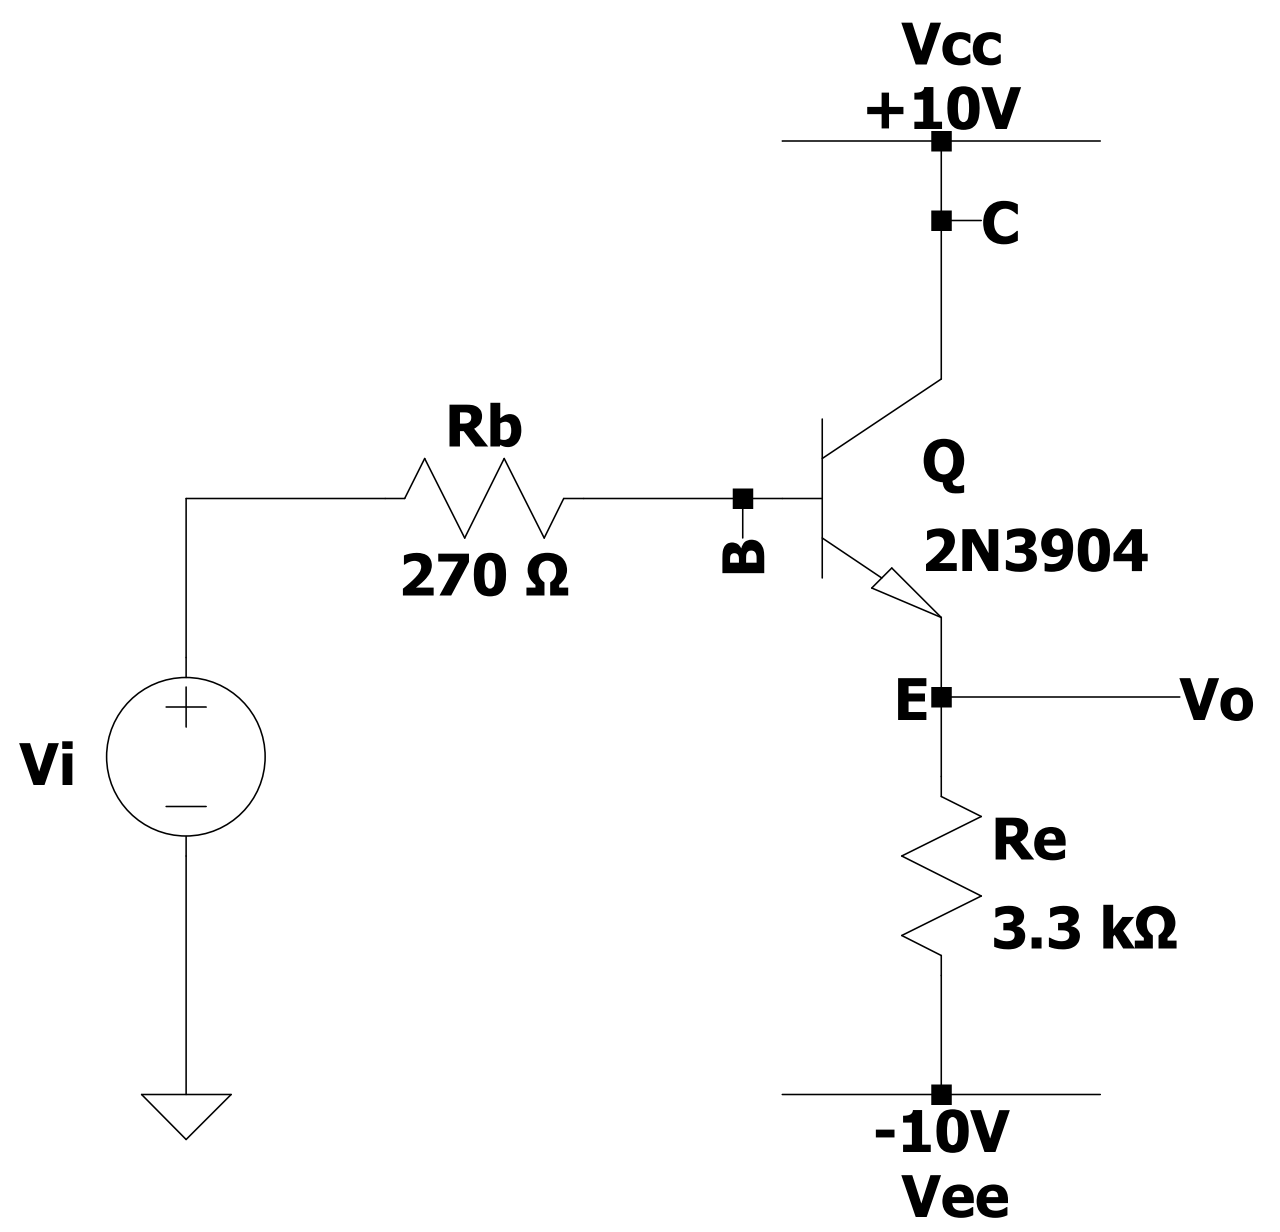
\includegraphics[height=10cm]{immagini/EFv1}
\caption{Schema dell'Emitter follower ad alimentazione duale.}
\end{figure}
\subsection{Analisi del punto di lavoro} 
Nell'analisi del punto di lavoro bisogna spegnere i generatori di segnale e sostituirli con un cortocircuito se sono generatori di tensione, oppure con un circuito aperto se sono generatori di corrente. I condensatori sono sostituiti con un circuito aperto e gli induttori con un cortocircuito. Successivamente si va a determinare la tensione di ogni nodo e la corrente che scorre in ogni ramo. 
\begin{figure}[h]
\centering
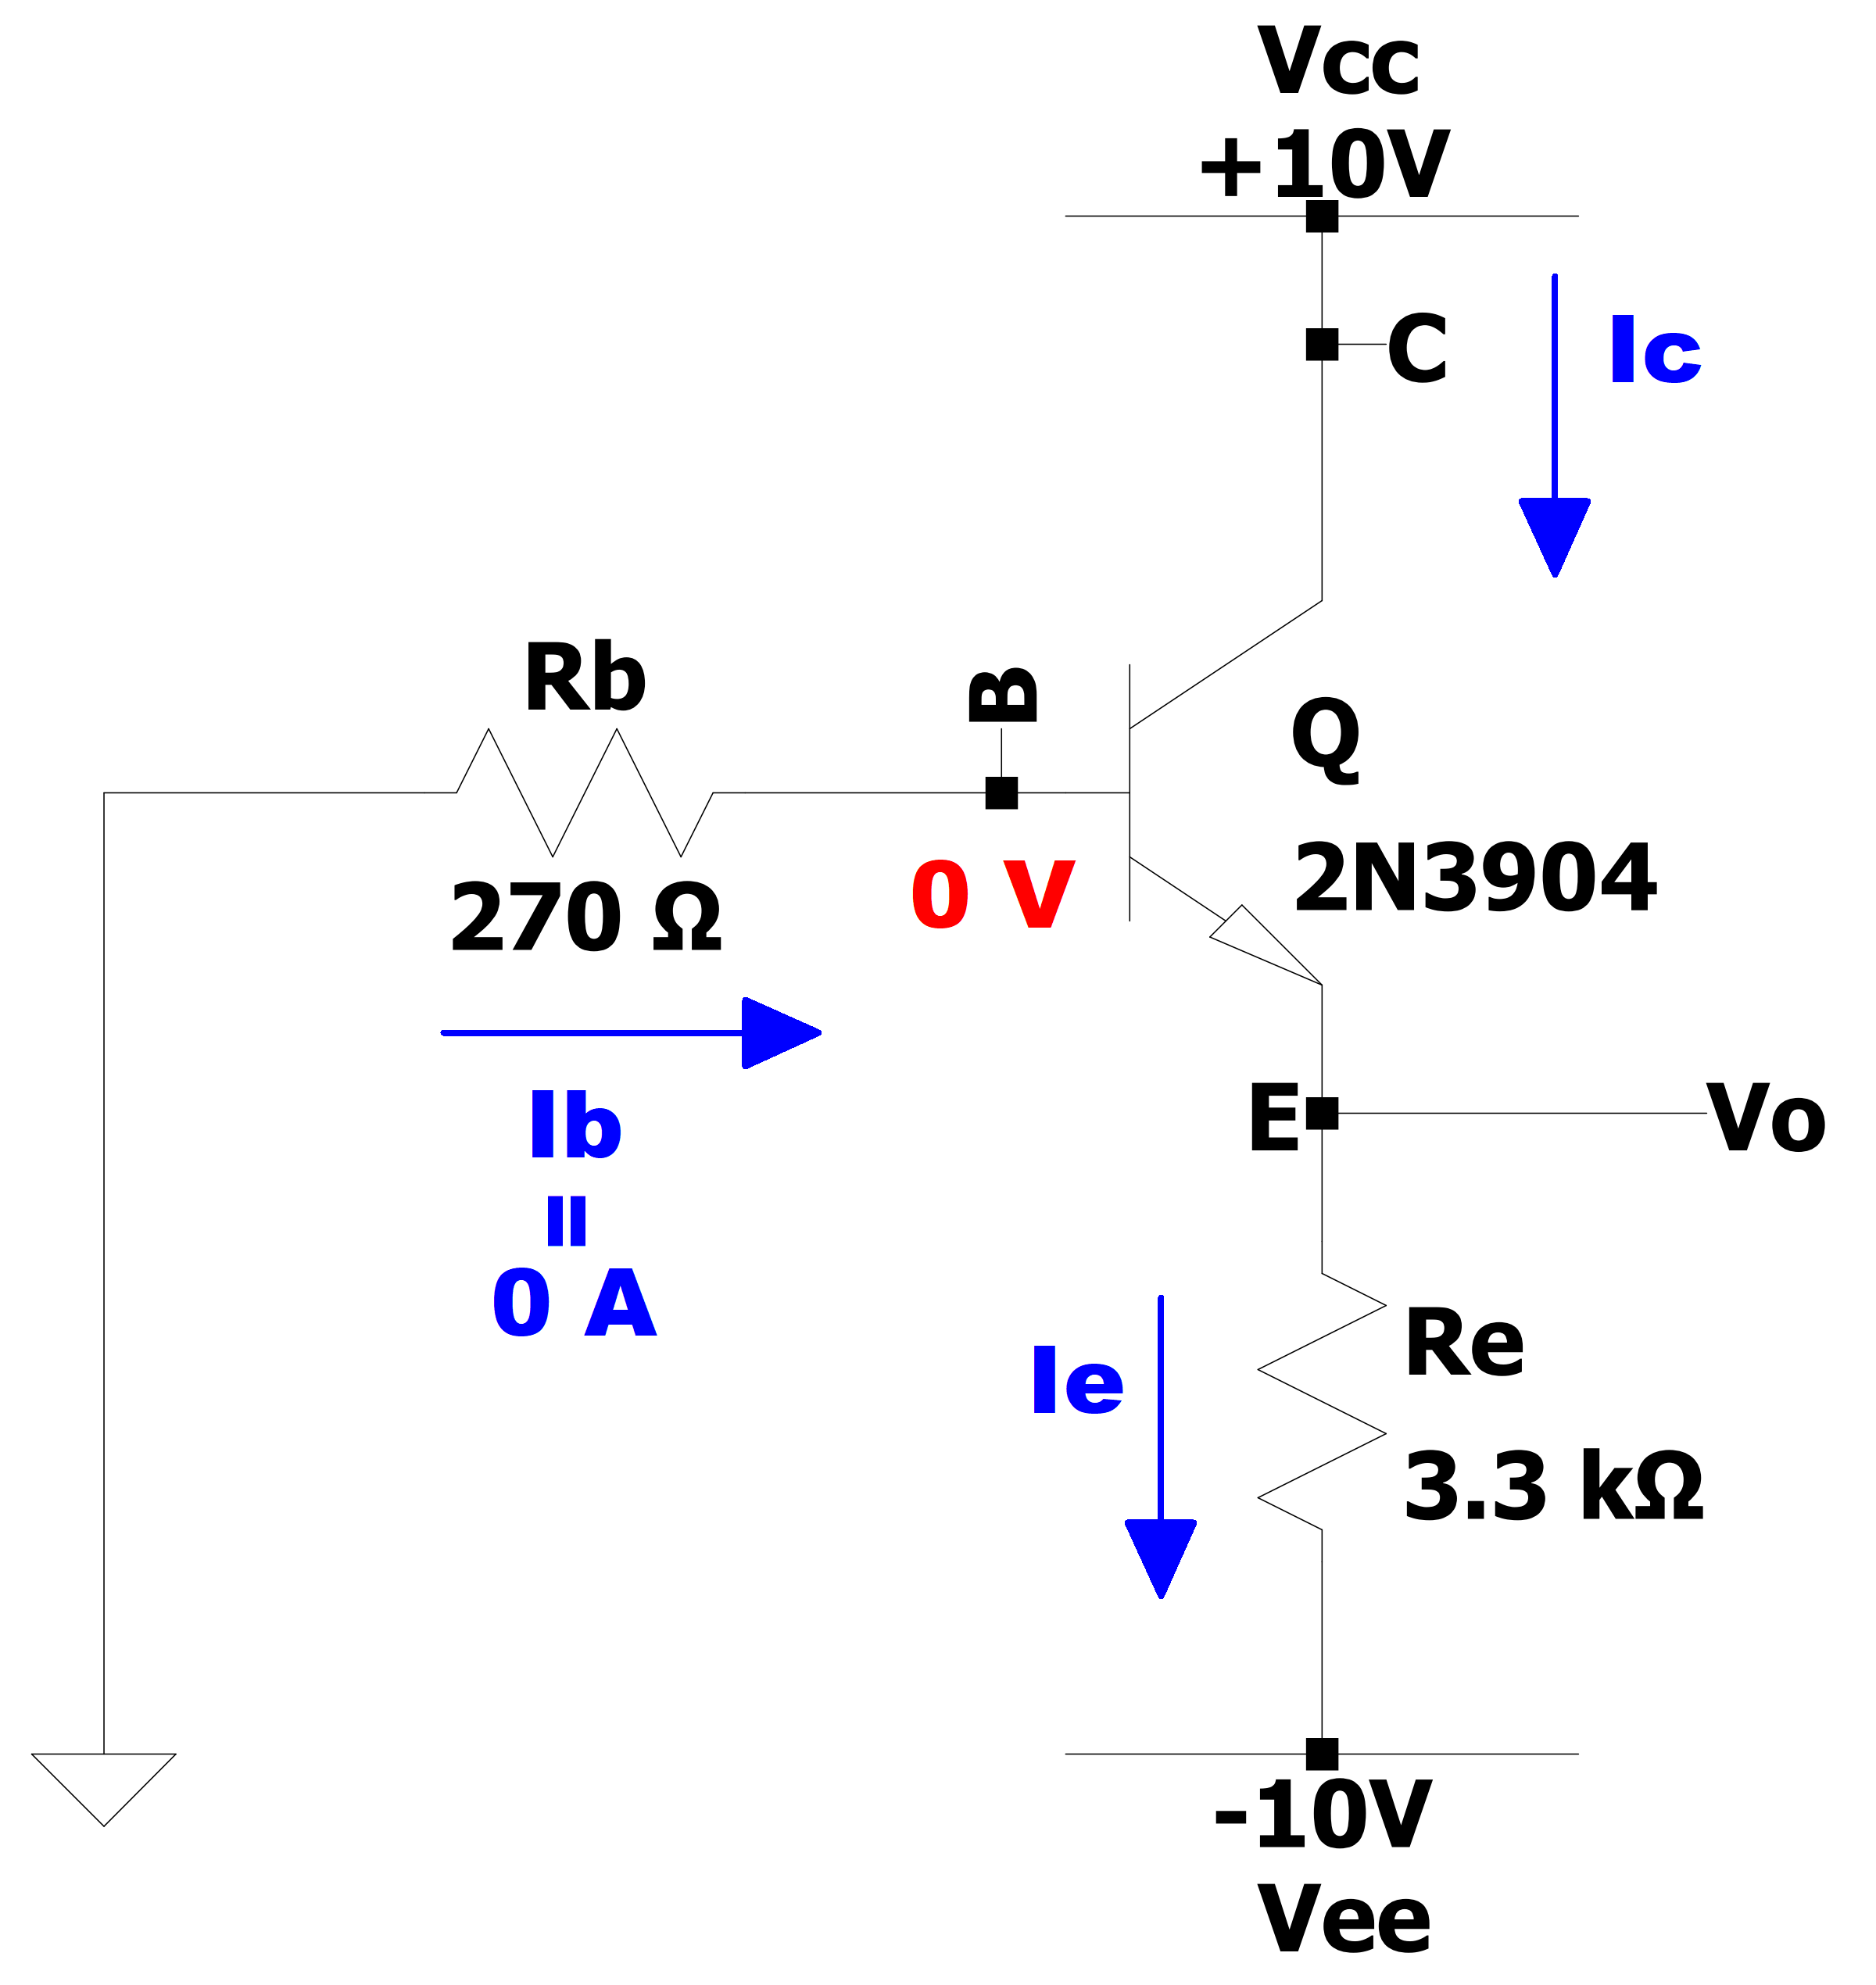
\includegraphics[height=10cm]{immagini/EFv1_pl}
\caption{Analisi del punto di lavoro dell'Emitter follower ad alimentazione duale.}
\label{figura:EFv1_pl}
\end{figure}
\\Come si vede nell'immagine~\ref{figura:EFv1_pl}, il generatore di segnale $v_{i}$ viene sostituito con un cortocircuito, quindi la resistenza $R_{B}$ si trova fra massa e la base del transistor \textit{Q}. In questo caso non dobbiamo apportare altre modifiche al circuito originale. 
\\Nell'analisi utilizziamo il modello ideale del transistor, perciò assumiamo che $\displaystyle{\beta\rightarrow\infty}$ e che $I_{B}=0A$, di conseguenza la corrente che fluisce nella resistenza è nulla, perciò, per la legge di Ohm, sarà nulla anche la caduta di tensione ai suoi capi, quindi si ricava che $V_{B}=0V$. 
\\Dal bilancio di correnti del  transistor (lo trattiamo come se fosse un nodo) otteniamo che $I_C+I_B=I_E$, ma dato che $I_{B}$ è nulla, allora $I_C=I_E$.
\\Suppondendo che il transistor si trovi in regione attiva diretta, la tensione $V_{BE}$ fra la base e l'emettitore è pari a circa +0.7V perché la giunzione è polarizzata direttamente. Dato che sappiamo che $V_{B}=0V$, possiamo calcolare per differenza $V_{E}$, dunque $V_{E}=-0.7V$. Anche $V_o$ sarà pari a questo valore dato che l'uscita viene prelevata all'emettitore.
\\$V_C$ è pari alla tensione di alimentazione positiva, perciò $V_C=V_{CC}=10V$.
Dato che $V_{CB}>0V$, la giunzione base-collettore è polarizzata inversamente, quindi l'ipotesi che il transistor si trovi in regione attiva diretta è verificata. 
\\Ora possiamo calcolare la corrente di emettitore con la legge di Ohm: 
\\[2pt]\indent$\displaystyle{V_E-V_{EE}=R_E\cdot I_E \rightarrow I_E=I_C=\frac{V_E-V_{EE}}{R_E}=\frac{-0.7V-(-10V)}{3.3k\Omega}=2.818mA}$
\\[2pt]Il circuito è ora completamente risolto, come ultima cosa si può calcolare la transconduttanza che ci servirà successivamente per l'analisi di piccolo segnale. La transconduttanza è definita come rapporto tra la corrente di collettore stazionaria $I_C$ e la tensione termica $V_T$, che a temperatura ambiente vale circa 26mV. 
\\[2pt]In formule: $\displaystyle{g_m=\frac{I_C}{V_T}=\frac{2.818mA}{26mV}=0.108 \frac{A}{V}}$.
\\[3pt]In tabella \ref{table:EFv1_pl} sono riassunte tutte le grandezze ricavate dall'analisi del punto di lavoro. 
\begin{table}[h]
	\centering
	\begin{tabular}{c|c|c|c|c|c|c}
		\hline
		\textbf{V\ped{B}[V]} & \textbf{V\ped{C}[V]} & \textbf{V\ped{E}[V]} & \textbf{I\ped{B}[A]} & \textbf{I\ped{C}[mA]} & \textbf{I\ped{E}[mA]} & \textbf{g\ped{m}[A/V]} \\ 
		\hline
		0 & 10 & -0.7 & 0 & 2.818 & 2.818 & 0.108\\ 
		\hline
	\end{tabular}
	
\caption{Riassunto delle grandezze ricavate dall'analisi del punto di lavoro del circuito.}
\label{table:EFv1_pl}
\end{table}
\subsection{Analisi di piccolo segnale} 
Nell'analisi di piccolo segnale bisogna spegnere i generatori di grandezze continue e sostituirli con un cortocircuito se sono generatori di tensione, oppure con un circuito aperto se sono generatori di corrente. Per analisi approssimate, i condensatori sono sostituiti con un cortocircuito e gli induttori con un circuito aperto; per analisi più accurate, invece, non vengono sostituiti e si utilizza la loro impedenza per risolvere il circuito. Infine, i transistor vengono sostituiti con il loro modello per piccolo segnale. Successivamente si va a determinare la tensione di ogni nodo e la corrente che scorre in ogni ramo, esattamente come avveniva per l'analisi del punto di lavoro. 
\begin{figure}[h]
\centering
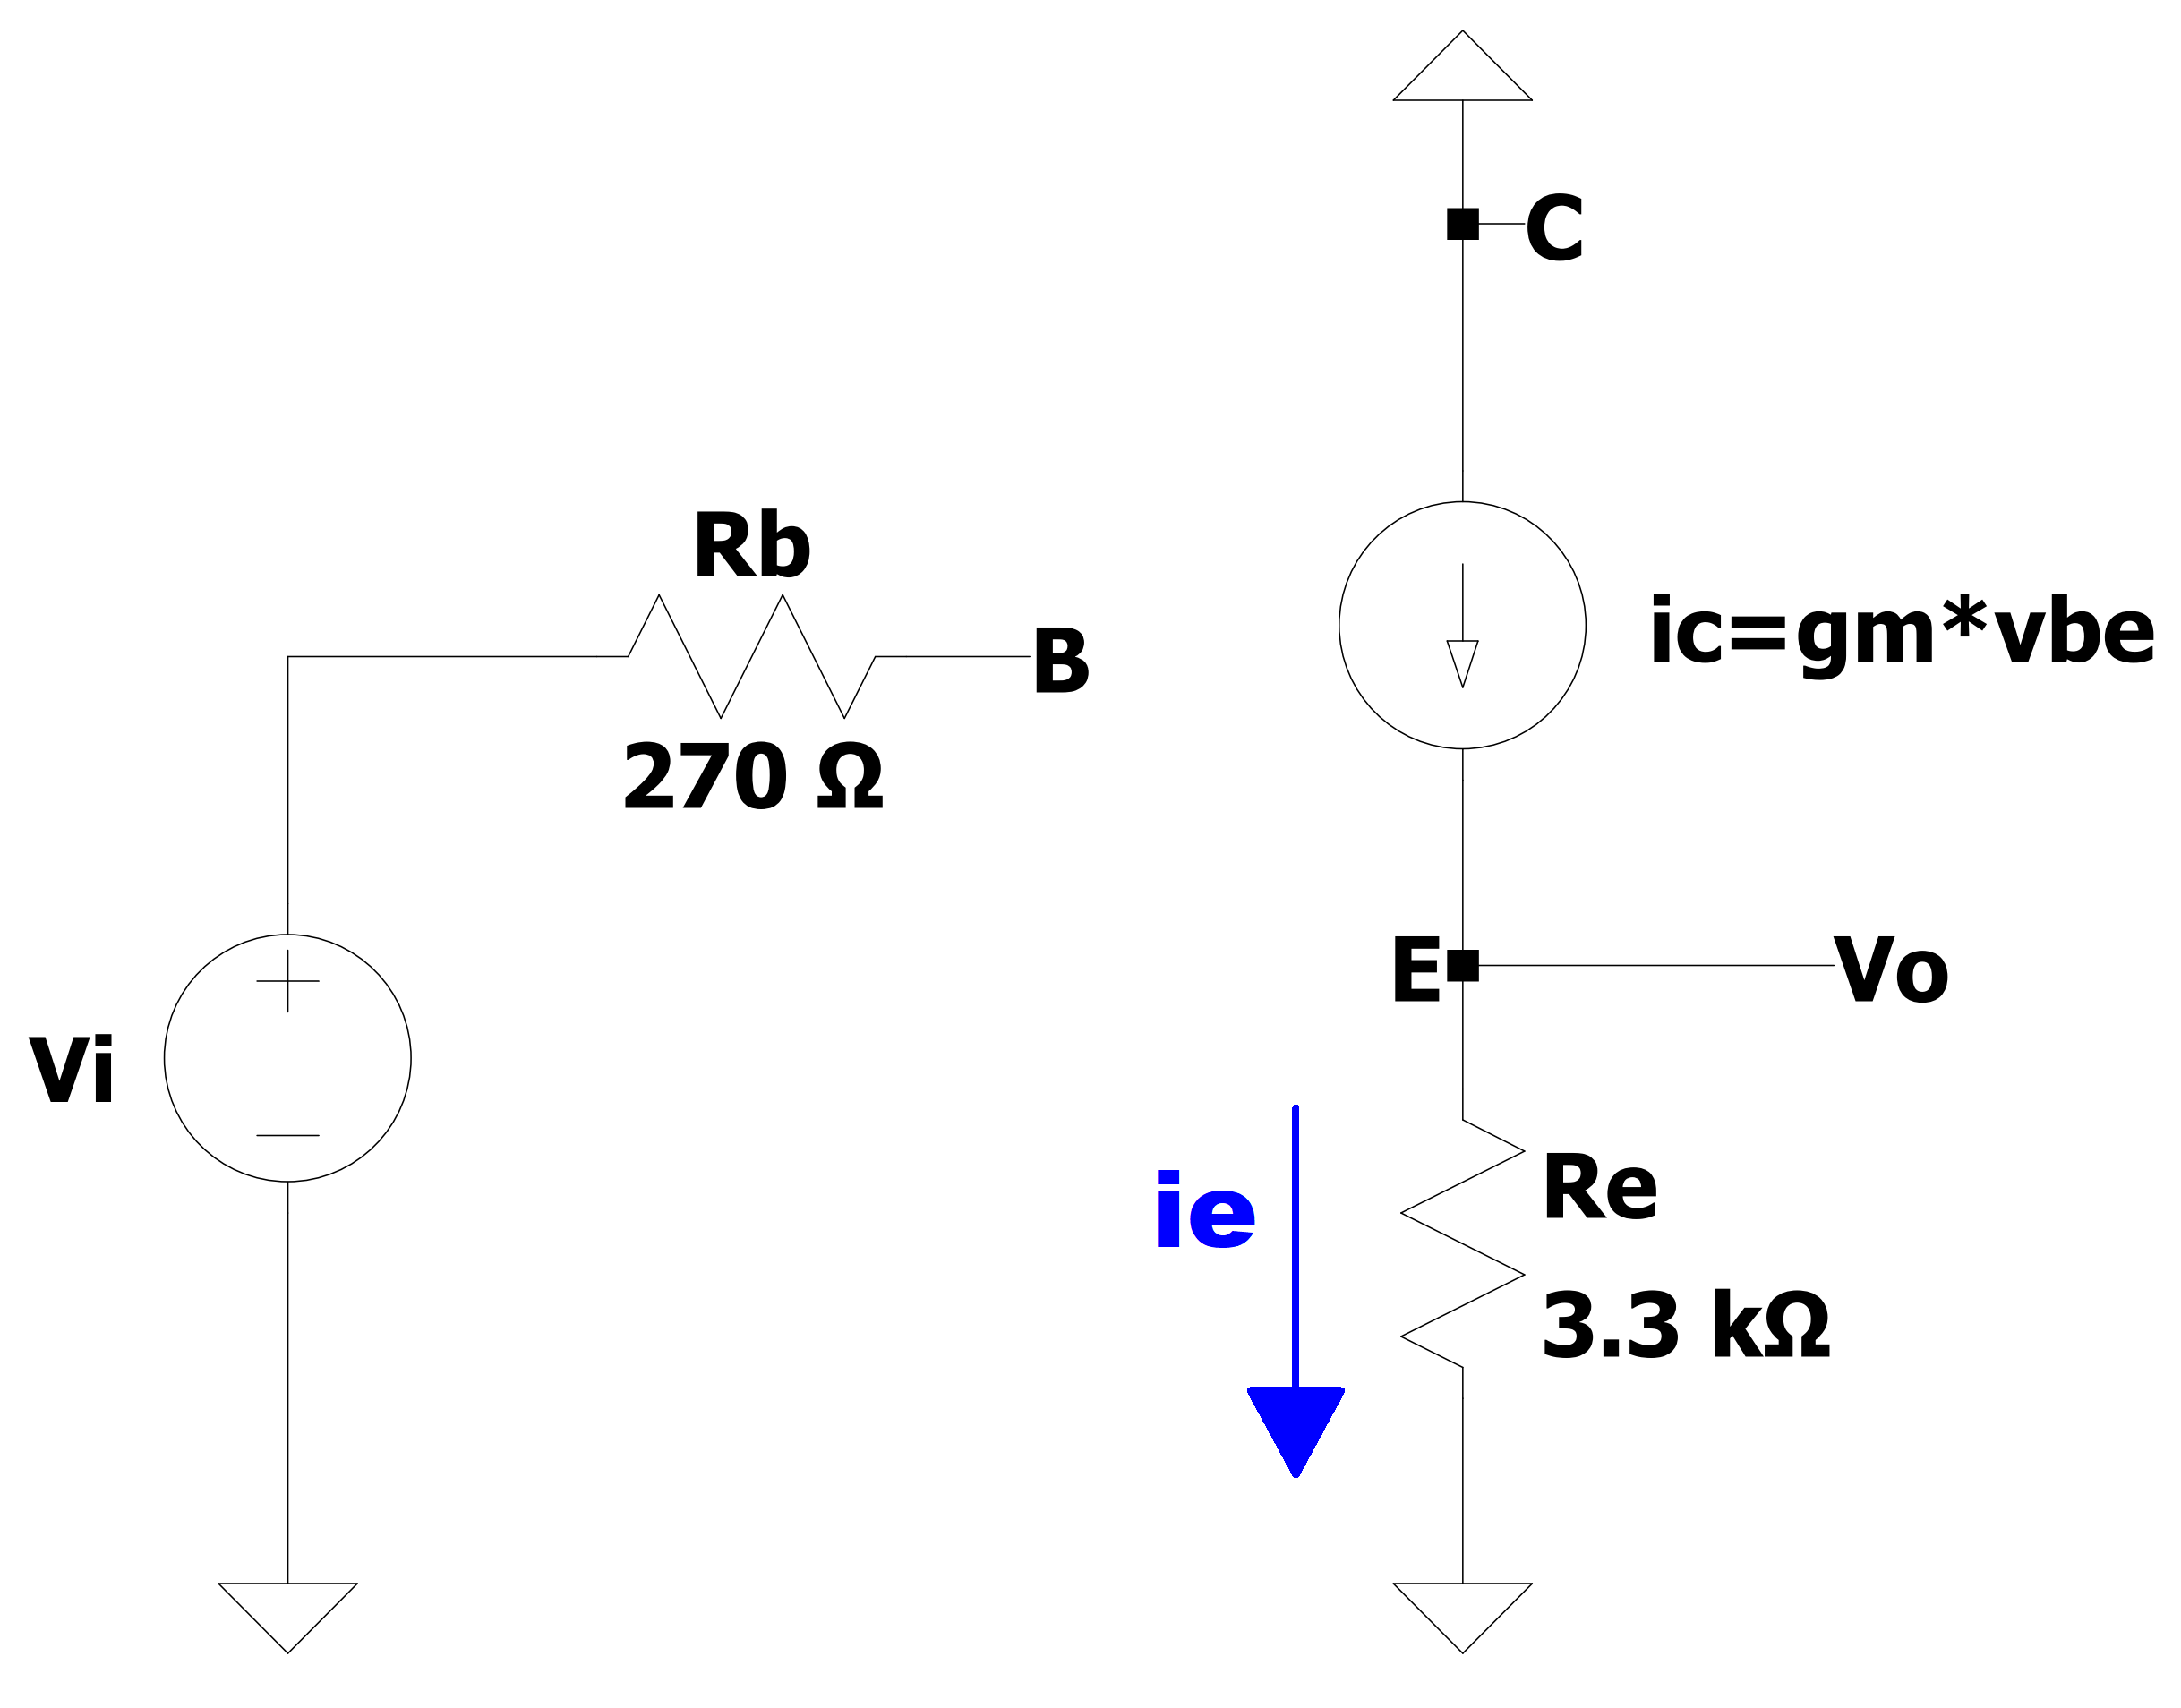
\includegraphics[height=9.6cm]{immagini/EFv1_ps}
\caption{Analisi di piccolo segnale dell'Emitter follower ad alimentazione duale.}
\label{figura:EFv1_ps}
\end{figure}
\\Come si può notare dalla figura~\ref{figura:EFv1_ps}, il BJT viene sostituito con il modello per piccolo segnale a bassa frequenza, quindi il terminale di base risulta isolato dal collettore e dall'emettitore, invece questi due terminali sono collegati attraverso un generatore di corrente di valore pari al prodotto fra la transconduttanza $g_m$ e la tensione $v_{BE}$.
\\Dato che la base del transistor è isolata, nel circuito di sinistra non circola corrente, perciò non c'è caduta di tensione sulla resistenza $R_B$, quindi la tensione $v_B$ risulta pari alla tensione applicata in ingresso con il generatore $v_i$.
\\Abbiamo già detto che $i_C=g_m\cdot v_{BE} = g_m(v_B-v_E) $. Ma dato che $v_B=v_i$ e $v_E=v_o$, la formula precedente per il calcolo della corrente di collettore si può riscrivere come $i_C=g_m(v_i-v_o)$.
\\[2pt]Ricaviamo $i_E$ con la legge di Ohm: 
$\displaystyle{i_E=\frac{v_E-0V}{R_E}=\frac{v_o}{R_E}}$.
\\[2 pt] Dal bilancio delle correnti al nodo E otteniamo che $i_C=i_E$. Sostituendo alle due correnti l'espressione ricavata ai punti precedenti ricaviamo la seguente eqauazione:
\\[2pt]\indent $\displaystyle{g_m(v_i-v_o)=\frac{v_o}{R_E}}$.
\\[2pt] A questo punto possiamo ricavare la funzione di trasferimento del circuito manipolando l'espressione ottenuta in precedenza. Questa risulta:
\\[2pt]\indent $\displaystyle{\frac{v_o}{v_i}=\frac{g_mR_E}{1+g_mR_E}\simeq1}$ per $g_mR_E\gg 1$. 
\\[2pt]Allora, si può dire che $v_o=v_i$, ovvero il circuito si comporta come un buffer, come si era già accennato nell'introduzione del circuito.
\\
\subsection{Componenti e misure} 
\section{Seconda versione} % alimentazione singola
\subsection{Analisi del punto di lavoro} 
\subsection{Analisi di piccolo segnale}  % versione base + versione partitore + versione condensatore
\subsection{Componenti e misure} 


%----------------------------------------------------------------------------------------
%	CIRCUITO 2: COMMON EMITTER AMPLIFIER
%----------------------------------------------------------------------------------------
\clearpage
\newpage
\chapter{Circuito 2: Common Emitter Amplifier}
\section{Introduzione} 
\section{Prima versione} % senza degenerazione emitter, solo trattazione teorica non realizzato in lab
\subsection{Schema} %?mettere
\subsection{Analisi del circuito} 
\section{Seconda versione} % con degenerazione emitter, alimentazione duale
\subsection{Analisi del punto di lavoro} 
\subsection{Analisi di piccolo segnale} 
\subsection{Componenti e misure} 
\section{Terza versione} % con degenerazione emitter, alimentazione singola (in piccolo segnale aggiungi già il condensatore)
\subsection{Analisi del punto di lavoro} 
\subsection{Analisi di piccolo segnale}  
\subsection{Componenti e misure} 


%----------------------------------------------------------------------------------------
%	CIRCUITI 3 E 4: AMPLIFICATORE OPERAZIONALE \mu A741
%----------------------------------------------------------------------------------------
\clearpage
\newpage
\chapter{Circuiti 3 e 4: Amplificatore operazionale \textmu A741}
\section{Introduzione} 
\section{Amplificatore invertente} 
\subsection{Schema} %?mettere
\subsection{Analisi del circuito} 
\subsection{Componenti e misure} 
\section{Integratore} 
\subsection{Schema} %?mettere
\subsection{Analisi del circuito} 
\subsection{Componenti e misure} 





%----------------------------------------------------------------------------------------

\end{document}
